\documentclass[12pt,oneside]{uhthesis}
\usepackage{subfigure}
\usepackage[ruled,lined,linesnumbered,titlenumbered,algochapter,spanish,onelanguage]{algorithm2e}
\usepackage{amsmath}
\usepackage{amssymb}
\usepackage{amsbsy}
\usepackage{caption,booktabs}
\captionsetup{ justification = centering }
%\usepackage{mathpazo}
\usepackage{float}
\setlength{\marginparwidth}{2cm}
\usepackage{todonotes}
\usepackage{listings}
\usepackage{xcolor}
\usepackage{multicol}
\usepackage{graphicx}
\floatstyle{plaintop}
\restylefloat{table}
\addbibresource{Bibliography.bib}
% \setlength{\parskip}{\baselineskip}%
\renewcommand{\tablename}{Tabla}
\renewcommand{\listalgorithmcfname}{Índice de Algoritmos}
%\dontprintsemicolon
\SetAlgoNoEnd

% parameter that is used in TeX's line breaking algorithm
\pretolerance=10000

\definecolor{codegreen}{rgb}{0,0.6,0}
\definecolor{codegray}{rgb}{0.5,0.5,0.5}
\definecolor{codepurple}{rgb}{0.58,0,0.82}
\definecolor{backcolour}{rgb}{0.95,0.95,0.92}

\lstdefinestyle{mystyle}{
    backgroundcolor=\color{backcolour},   
    commentstyle=\color{codegreen},
    keywordstyle=\color{purple},
    numberstyle=\tiny\color{codegray},
    stringstyle=\color{codepurple},
    basicstyle=\ttfamily\footnotesize,
    breakatwhitespace=false,         
    breaklines=true,                 
    captionpos=b,                    
    keepspaces=true,                 
    numbers=left,                    
    numbersep=5pt,                  
    showspaces=false,                
    showstringspaces=false,
    showtabs=false,                  
    tabsize=4
}

\lstset{style=mystyle}

\title{Sistema de subasta a ciegas sobre Quorum}
\author{\\\vspace{0.25cm}Alben Luis Urquiza Rojas}
\advisor{\\\vspace{0.25cm}Dr.C. Yaidir Mustelier Ruiz} %\\\vspace{0.2cm}Nombre del segundo tutor
\degree{Licenciado en Ciencia de la Computación}
\faculty{Facultad de Matemática y Computación}
\date{Fecha: Noviembre 2022\\\vspace{0.25cm} \href{https://github.com/ic-matcom/blind-auction-quorum}{github.com/ic-matcom/blind-auction-quorum}}
\logo{Graphics/uhlogo}
\makenomenclature

\renewcommand{\vec}[1]{\boldsymbol{#1}}
\newcommand{\diff}[1]{\ensuremath{\mathrm{d}#1}}
\newcommand{\me}[1]{\mathrm{e}^{#1}}
\newcommand{\pf}{\mathfrak{p}}
\newcommand{\qf}{\mathfrak{q}}
%\newcommand{\kf}{\mathfrak{k}}
\newcommand{\kt}{\mathtt{k}}
\newcommand{\mf}{\mathfrak{m}}
\newcommand{\hf}{\mathfrak{h}}
\newcommand{\fac}{\mathrm{fac}}
\newcommand{\maxx}[1]{\max\left\{ #1 \right\} }
\newcommand{\minn}[1]{\min\left\{ #1 \right\} }
\newcommand{\lldpcf}{1.25}
\newcommand{\nnorm}[1]{\left\lvert #1 \right\rvert }
\renewcommand{\lstlistingname}{Ejemplo de código}
\renewcommand{\lstlistlistingname}{Ejemplos de código}

\begin{document}

\frontmatter
\maketitle

% \begin{dedication}
    Dedicación
\end{dedication}
% \begin{acknowledgements}
    Agradecimientos
\end{acknowledgements}
% \begin{opinion}
    Opiniones de los tutores
\end{opinion}
% \begin{resumen}
	Las subastas son un mecanismo de venta cada día más usado. Con el auge de las tecnologías de la información, sistemas de pago electrónico y de un mundo interconectado, a través de internet, cada vez se hace un mayor uso de subastas electrónicas. Por esta razón, se hace necesario proponer nuevos protocolos y mecanismos para incrementar la seguridad de estos sistemas y protegerlos de hackers que explotan vulnerabilidades de seguridad en las plataformas en línea, pero también proteger a los usuarios de subastadores malintencionados que pueden terminar siendo estafadores, este último problema cada vez más latente en la actualidad. En la presente investigación se hace un estudio de los protocolos de una subasta en particular, las subastas a ciegas sobre blockchain. Luego de revisar y valorar las propuestas de la literatura consultada sobre el tema, se hace una propuesta e implementación de un contrato inteligente que permite la realización de una variante de subasta holandesa (a ciegas), en el lenguaje de programación Solidity, que pudiera ser utilizada en el Mercado de Deuda Pública de Cuba. Se valora, además, la factibilidad de la blockchain de Quorum como blockchain objetivo para desplegar la propuesta presentada. Y por último, se realiza un despliegue del contrato inteligente en una red blockchain local, en la cual se realizaron pruebas que fueron satisfactorias, llegando a la conclusión de que la propuesta es factible y puede ser empleada para realizar subastas a ciegas.

\end{resumen}

\begin{abstract}
	Auctions are an increasingly used sales mechanism. With the rise of information technologies, electronic payment systems and an interconnected world, through the Internet, there is increasing use of electronic auctions. For this reason, it is necessary to propose new protocols and mechanisms to increase the security of these systems and protect them from hackers who exploit security vulnerabilities in online platforms, but also protect users from malicious auctioneers who may end up being scammers. This last problem is increasingly common today. In the present investigation, a study is made of the protocols of a particular auction, blind auctions on blockchain. After reviewing and evaluating the proposals of the literature consulted on this topic, a proposal and implementation of a smart contract is made that allows the realization of a variant of the Dutch (blind) auction, in the Solidity programming language, which could be used in the Cuban Public Debt Market. In addition, the feasibility of the Quorum blockchain as the blockchain to deploy the presented proposal is assessed. And finally, a deployment of the smart contract is carried out in a local blockchain network, in which tests were carried out that were satisfactory, reaching the conclusion that the proposal is feasible and can be used to carry out blind auctions.
\end{abstract}

\tableofcontents
\listoffigures
% \listoftables
% \listofalgorithms
\lstlistoflistings

\mainmatter

\chapter*{Introducción}\label{chapter:introduction}
\addcontentsline{toc}{chapter}{Introducción}

% \hspace*{}

  Cuando el 31 de octubre de 2008 Satoshi Nakamoto publicó el artículo \textit{Bitcoin: A Peer-to-Peer Electronic Cash System} (documento 
  técnico original de la bien conocida y primera criptomoneda: Bitcoin) , creó las bases de una tecnología que 
  está revolucionando al mundo, y el autor no se refiere al que bien pudiera ser el sistema de pago que sustituya al dólar y al dinero 
  \textit{fiat} en un futuro, sino a la \textit{blockchain} ~\parencite{satoshi2008}.
  
  \textit{Blockchain} se traduce como cadena de bloques. Básicamente, es un conjunto de tecnologías que permiten llevar un registro 
  seguro, descentralizado, sincronizado y distribuido de operaciones digitales, sin necesidad de la intervención de terceros 
  \parencite{solunion2021}.

  En ese sentido, la definición más completa es la dada por Don \& Alex Tapscott en su libro Blockchain Revolution
  ~\parencite{tapscott2016blockchain}: “un libro de 
  contabilidad digital incorruptible de transacciones económicas que se puede programar para registrar no solo transacciones financieras, 
  sino prácticamente todo lo que tiene valor”. Cada uno de los bloques de datos se encuentra protegido y vinculado entre sí 
  criptográficamente. Las transacciones no las verifica un tercero, sino la red 
  de nodos (computadores conectados a la red), que también es la que autoriza en consenso cualquier actualización en la \textit{blockchain} 
  \parencite{solunion2021}.

  A finales de 2013, Vitalik Buterin publica el que luego se convertiría en el documento técnico (\textit{white paper}) de Ethereum 
  \parencite{buterin2013}. Este joven, quien hasta ese momento era uno de los
  programadores involucrado en el ecosistema Bitcoin, había notado el potencial de la criptografía para el desarrollo de aplicaciones 
  descentralizadas. No obstante, su propuesta de crear un lenguaje de scripting para Bitcoin, que hiciera esto posible, no tuvo resonancia 
  suficiente. Fue entonces cuando se propuso el desarrollo de una red independiente, con su propia infraestructura, para el desarrollo de 
  un criptoactivo y una cadena de bloques capaz de soportar aplicaciones descentralizadas. Y el 30 de julio de 2015, Vitalik conjuntamente
  con otros programadores pusieron en línea la \textit{blockchain} de Ethereum \parencite{diaz2018}. 
  
  La red de Ethereum llevó a la práctica un nuevo concepto, los contratos inteligentes, en inglés conocidos como \textit{smart contracts}. 
  La definición más simple al respecto es que se trata de contratos que tienen la capacidad de cumplirse de forma automática una vez que 
  las partes han acordado los términos. Su nombre hace recordar a los contratos legales firmados en papel. Pero a pesar de que tienen 
  cosas en común, son totalmente diferentes. 

  Los contratos inteligentes son programas informáticos. No están escritos en lenguaje natural, sino en código virtual. Son un 
  tipo de software que se programa, como cualquier otro software, para llevar a cabo una tarea o serie de tareas determinadas de acuerdo a 
  las instrucciones previamente introducidas. Su cumplimiento, por tanto, no está sujeto a la interpretación de ninguna de las partes: si 
  el evento A sucede, entonces la consecuencia B se pondrá en marcha de forma automática. Su implicación legal ha caído -como toda la 
  tecnología relacionada a Bitcoin- en una zona gris. No se requiere de ningún intermediario de confianza (como una notaría), pues este 
  papel lo adopta el código informático, que asegurará sin dudas el cumplimiento de las condiciones. Por tanto, se reducen tiempo y costes 
  significativamente ~\parencite{smartcontract}. 

  % A smart contract is a computer program or a transaction protocol that is intended to automatically execute, control or document legally 
  % relevant events and actions according to the terms of a contract or an agreement.[1][2][3][4] The objectives of smart contracts are the 
  % reduction of need for trusted intermediators, arbitrations costs, fraud losses, as well as the reduction of malicious and accidental 
  % exceptions.[5][2]

  Las ventajas son obvias, y pueden reducirse a tres palabras: autonomía, seguridad y confianza. Utilizando contratos inteligentes ya no 
  resulta necesario recurrir a un tercero —como un abogado o un notario—, que además de que pueden provocar errores, ocasiona gastos 
  significativos. La \textit{blockchain} es capaz de resguardar la información en una red cifrada que puede consultarse desde cualquier lugar del 
  mundo, por lo que la velocidad y seguridad saltan a la vista.

  Con esta nueva tecnología se puede crear una gran cantidad de nuevas aplicaciones para hacer trámites y transacciones hasta ahora
  difíciles de realizar con las tecnologías existentes, o simplemente mejorar servicios gracias a la descentralización
  de la \textit{blockchain} y de los contratos inteligentes.

  Una de estas aplicaciones de los contratos inteligentes está dada a las subastas. Una subasta es una venta generalmente pública en la 
  que se adjudica una cosa, especialmente bienes o cosas de valor, a la persona que ofrece más dinero por ella. La \textit{blockchain} puede y 
  está cambiando, la manera en la que se hacen las subastas, ya sin necesidad de un subastador o de alguna entidad que haga de mediador. 
  Ya muchas casas de apuestas han actualizado sus políticas, para adaptarse a los nuevos métodos, de hacer subastas. 
  % https://tezro.com/
  % https://bitify.com/
  % https://nft.christies.com/  Founded in 1766, Christie’s is a world-leading art and luxury business.
  % https://portion.io/     Portion is the premier online marketplace connecting artists and collectors through Blockchain technology to 
  % easily sell, invest and own art and collectibles with complete transparency.
  % https://www.coindesk.com/markets/2021/07/09/sothebys-sells-rare-diamond-for-123m-in-crypto/

  Los mercados de deuda pública o de bonos soberanos(o del estado) siempre han hecho uso de subastas para hacer sus ventas. Con la
  \textit{blockchain} se abre una nueva puerta para una forma segura, eficiente y sencilla de efectuar estas subastas. 

  Específicamente, en el presente trabajo se estudian las subastas a ciegas. Una subasta a ciegas es aquella en la que solo el ofertante 
  sabe el monto de su oferta y nadie más. Él no conoce las ofertas de los demás y viceversa.

  La implementación de subastas a ciegas sobre \textit{blockchain} presupone una dificultad, pues toda información que se almacena es pública y 
  verificable por cualquiera que esté conectado a la red de nodos. La solución a esto podría ser el cifrado de las ofertas que hacen 
  los pujadores. Por tanto, el problema consiste en la selección del algoritmo adecuado para el desarrollo de un sistema de 
  subasta a ciegas.

  El problema científico abordado en esta investigación es: analizar algoritmos, criptográficos o no 
  criptográficos, para la 
  realización de subastas a ciegas. Que se enmarca en el objeto de investigación: subastas electrónicas. 
  El \textbf{objetivo} general de 
  este trabajo es el diseño e implementación de un conjunto de algoritmos que permita el desarrollo de 
  subastas a ciegas sobre Quorum 
  (Quorum es una \textit{blockchain} basada en Ethereum). Este objetivo delimita el siguiente campo de 
  acción: implementación de subastas a ciegas sobre Quorum.

  Para lograr el objetivo general se definen los siguientes objetivos específicos:

  \begin{enumerate}
    \item Identificar las soluciones técnicas y tecnologías que se emplean para el desarrollo de aplicaciones relacionadas 
    con subasta electrónica.

    \item Valorar las posibilidades de Quorum como plataforma para el desarrollo de aplicaciones de este tipo.

    \item Estudio de Solidity como lenguaje de programación para el desarrollo de contratos inteligentes sobre Quorum.

    \item Implementar contratos inteligentes (algoritmos) que permitan efectuar subastas a ciegas.

  \end{enumerate}

  La memoria escrita está organizada en tres capítulos.
  En el Capítulo 1 se aborda el tema de las subastas, qué beneficios presenta la \textit{blockchain} para el desarrollo de subastas y 
  una comparación entre algunos tipos de protocolos de subastas a ciegas sobre \textit{blockchain}. En el Capítulo 2 se explica la 
  utilización de la \textit{blockchain} de Quorum para el desarrollo de un sistema de subastas a ciegas. El Capítulo 3 está dedicado a la 
  evaluación de los resultados y mostrar el desempeño del método propuesto. Finalmente, se dan las conclusiones de la investigación, 
  recomendaciones, así como la bibliografía y los anexos necesarios para la mejor comprensión de la propuesta.

\chapter{Subastas y blockchain}\label{chapter:chapter1}

\hspace*{}

\section{Subastas}
  
  \hspace*{}

  Una subasta es el proceso de comprar y vender bienes o servicios. Este proceso implica ofrecer artículos 
  para vender, esperar que sean enviadas las ofertas y vender los bienes a la mayor oferta, bajo la supervisión
  de un subastador \parencite{krishna}.

  % An auction is a process of buying and selling goods or services. This process involves offering items 
  % for bidding, waiting for bids to be accepted, and then selling goods to the highest bidder under the 
  % supervision of an auctioneer. [5]

  Por la relevancia del término, se considera importante revisar qué definiciones formales de "subasta" existen:

  - Definición de la RAE: %(Real Academia Española)
  1. f. Venta pública de bienes o alhajas que se hace al mejor postor, y regularmente por mandato y con intervención de un juez u otra 
  autoridad.
  2. f. Adjudicación de una contrata, generalmente de servicio público, como la ejecución de una obra, el suministro de provisiones, etc., 
  a quien presenta la propuesta más ventajosa \parencite{raesubasta}.

  - Economipedia:
  Una subasta es un procedimiento de venta donde los interesados compiten entre sí para adjudicarse el bien o servicio a ser subastado 
  \parencite{economipediasubasta}.

  \subsection{Tipos de subastas} \hspace*{}

    Las subastas pueden clasificarse en diferentes tipos. A continuación se resumen las características de las más conocidas.

    - English Auction (Subasta Inglesa o ascendente): Este es el tipo de subasta más conocido. Las pujas comienzan con un precio bajo, y se 
    incrementan progresivamente a medida que se solicitan pujas más altas, hasta que se cierra la subasta o 
    no se reciben pujas más altas. A menudo el vendedor fija un precio de reserva por debajo del cual el 
    artículo no se vende y la subasta se cancela. Permite a un vendedor asegurar el precio más alto para un 
    artículo.

    - Dutch Auction (Subasta holandesa o descendente): El precio empieza alto y va bajando hasta que algún participante está 
    dispuesto a pagar el precio, y este es el que gana y paga el último precio que se menciona.

    \textbf{- Blind Auction (Subasta a ciegas o de sobre cerrado)}: También conocida en la literatura como First-Price sealed-bid auction(FPSBA)
    En este tipo de subasta, todas las ofertas se envían simultáneamente y nadie sabe que oferta hizo el resto
    de los participantes. Gana el que mayor oferta hizo y paga esa cantidad al vendedor.

    - Vickrey Auction (Subasta Vickrey): Conocida también en la literatura en inglés como sealed-bid second-price auction (SBSPA)
    % subasta de segundo precio de puja sellada
    . Es un tipo de subasta de puja sellada, donde los oferentes presentan ofertas por escrito sin conocer la oferta de las otras 
    personas en la subasta, y en la que gana el postor más alto, pero el precio que paga este es la segunda oferta más alta \parencite{economipediasubasta}.   
    % Este tipo de subasta fue descrito por primera vez por el profesor William Vickrey en la Universidad de Columbia en 1961 
    % % Vickrey, William (1961). «Counterspeculation, Auctions, and Competitive Sealed Tenders». The Journal of Finance 16 (1): 8-37. doi:10.1111/j.1540-6261.1961.tb02789.x.
    % , aunque había sido utilizada por coleccionistas de sellos desde 1893. Este tipo de subasta es estratégicamente similar a una 
    % subasta inglesa e incentiva a que los oferentes presenten ofertas iguales a su verdadera valoración del objeto subastado.
    % Las Subastas Vickrey son muy estudiadas en la literatura económica, pero no son particularmente comunes en la práctica.

    - All-pay auction (Subasta americana): es como la subasta inglesa, pero, todos los postores deben pagar la oferta que hacen, pero solo el que realiza 
    la mejor oferta obtiene el producto.
    % https://www.investopedia.com/terms/a/all-pay-auction.asp

    - Silent auction (Subasta Silenciosa):
    Las pujas se escriben en hojas de papel. Al final de la subasta, la puja más alta se adjudica la subasta. Este tipo de subasta se 
    utiliza frecuentemente en eventos de beneficencia, en los que se subastan muchos objetos simultáneamente, y se "cierra" a una hora 
    predeterminada común a todos los objetos. La subasta es "silenciosa" porque no hay subastador y los pujadores escriben sus pujas en 
    una hoja que usualmente se deja en una mesa cercana al objeto. En las subastas de beneficencia, las hojas usualmente indican una 
    puja inicial mínima, los incrementos que se pueden hacer sobre dicha puja mínima y una cantidad, llamada "puja garantizada" que si 
    se paga se obtiene el objeto de forma inmediata. Otras variaciones de este tipo de puja pueden incluir pujas selladas. El pujador 
    con la puja más alta paga el precio que indicó en su hoja y obtiene el bien \parencite{investopedia}.

    - Reverse auction (Subasta inversa o reversa):
    Es un tipo de subasta en la que se invierten los papeles de comprador y el vendedor. En una subasta ordinaria, los compradores compiten 
    para obtener un bien o servicio, ofreciendo precios cada vez más altos. En una subasta inversa, los vendedores compiten para obtener 
    negocio del comprador y los precios suelen disminuir a medida que los vendedores hacen sus ofertas.
      % https://es.wikipedia.org/wiki/Subasta_inversa

    - Candle Auction (Subasta de velas):
    Es una variación de la subasta típica inglesa que se hizo popular en los siglos XVII y XVIII. En una subasta de velas, el final 
    de la subasta se indica con el vencimiento de la llama de una vela, que tenía la intención de garantizar que nadie pudiera saber 
    exactamente cuándo terminaría la subasta y hacer una oferta de último segundo. A veces, se utilizaron otros procesos impredecibles, 
    como una carrera a pie, en lugar de la expiración de una vela \parencite{patten1970}.
    % https://en.wikipedia.org/wiki/Candle_auction

    - Double Auction (Subasta Doble):
    Una doble subasta es un proceso de compra y venta de bienes cuando los compradores potenciales y los posibles vendedores presenten 
    simultáneamente sus ofertas, su demanda, los precios de una casa de subastas, y luego un subastador elige algún precio \textit{p} que 
    equilibra el mercado: todos los vendedores que solicitaron menos de \textit{p} venden y todos los compradores que pujaron más de 
    \textit{p} compran a este precio \textit{p} \parencite{friedman1992}.
    % https://en.wikipedia.org/wiki/Double_auction
    
    Hay algunos otros tipos de subasta, pero mucho menos conocidas. Como fue explicado en la Introducción la presente investigación se 
    enfoca precisamente en subastas a ciegas.

  \subsection{Mercado de deuda} \hspace*{}

    El mercado de deuda o bonos es donde se emiten y negocian los títulos de deuda, cuando los participantes no están en condiciones o no 
    desean pedir préstamos o créditos a la banca. En él participan el Gobierno Federal, los gobiernos estatales o locales y las empresas 
    paraestatales o privadas que necesitan financiamiento, ya sea para realizar un proyecto de inversión o para mantener sus propias 
    actividades. Una parte de este mercado se conoce como mercado del dinero, que es en donde se intercambian los bonos que por su corto 
    plazo, liquidez y alta seguridad se pueden considerar sustitutos del dinero.

    El mercado de deuda también se conoce con otros nombres dependiendo del tipo de instrumentos de deuda negociado. Por ejemplo, si en el 
    mercado se negocian principalmente instrumentos de deuda que pagan una tasa fija, entonces se denomina mercado de renta fija, mercado 
    de renta variable, mercados de deuda internacional, de deuda pública, etc. En términos generales, para que una persona pueda comprar 
    o vender títulos de deuda es necesario que acudan a un banco o a una casa de bolsa para que dichas instituciones puedan efectuar las 
    transacciones necesarias a nombre de esta persona \parencite{bancomexico}.

    En este caso vamos a estar refiriéndonos específicamente al mercado de deuda pública o el mercado de bonos del Estado. Un bono del 
    Estado es un tipo de inversión basada en deuda, en que le prestas dinero a un gobierno a cambio de una tasa de interés acordada. Los 
    gobiernos los utilizan para generar fondos que pueden gastar en nuevos proyectos o infraestructura, mientras que los inversores 
    pueden usarlos a fin de que se les pague un retorno establecido en intervalos periódicos.

    Cuando compras un bono del Estado, le prestas al Gobierno una cantidad acordada de dinero durante un período también acordado. A 
    cambio de esto, el Gobierno te devuelve el dinero con un nivel establecido de interés de forma periódica, lo que se conoce como 
    cupón. De esta manera, los bonos conforman un activo de ingreso fijo.

    Cuando el bono venza, se te devolverá tu inversión original (denominada principal). El día en que recibes el valor de capital 
    adeudado se conoce como la fecha de vencimiento. Diferentes bonos tienen distintas fechas de vencimiento; por ejemplo, puedes 
    comprar un bono que vence en menos de un año o uno que vence en 30 años o más.

    Algunos inversores dicen que los bonos del Estado son inversiones libres de riesgo. Dado que un gobierno siempre puede imprimir más 
    dinero para saldar sus deudas, teóricamente hablando, siempre se te devolverá tu dinero cuando venza el bono.

    En la realidad, esto es mucho más complicado. En primer lugar, los gobiernos no siempre pueden producir más capital. Incluso si es 
    que pudieran hacerlo, esto no evita que incumplan el pago de los préstamos. No obstante, aparte del riesgo crediticio, existen otros 
    posibles problemas de los cuales preocuparse con los bonos del Estado, por ejemplo, el riesgo de las tasas de interés, la inflación 
    y las divisas \parencite{igbonos}.

  \subsection{Mercado de Deuda Pública en Cuba} \hspace*{}

    Cuando en nuestra economía doméstica los gastos superan a los ingresos no nos queda más remedio que pedir prestado, de lo contrario 
    no podemos pagar lo que necesitamos o debemos. En otras palabras, tendríamos que disminuir o aplazar las compras. Al presupuesto del 
    Estado le sucede exactamente lo mismo y sus ausencias de dinero se llaman déficit fiscal. La deuda pública es la suma del déficit 
    fiscal del año, más las garantías que se activen en esos 12 meses (porque el presupuesto del Estado es garante de determinadas 
    operaciones económicas como inversiones en sectores priorizados) y las amortizaciones de deudas anteriores provenientes de los bonos 
    que se colocaron en lo años anteriores.

    Pero, ¿cómo se financia el déficit presupuestario? Esto ocurre mediante bonos soberanos de la República de 
    Cuba que emite el Ministerio de Finanzas y Precios (MFP) y que hasta el momento han sido adquiridos por el sistema bancario nacional.

    El Banco de Inversiones es el encargado de colocar, emitir y registrar la emisión. El MFP le solicita una emisión de bonos y este lo 
    coloca en el sistema bancario, y cada banco comercial (Banco de Crédito y Comercio, Popular de Ahorro y Metropolitano) adquiere el 
    monto que puede asumir. En caso de que los bancos no tengan suficiente liquidez para cubrir totalmente el bono, interviene el Banco 
    Central de Cuba(BCC) con la emisión de nuevos billetes.

    Hasta 2013 el déficit se financiaba solo de esta manera (con la emisión de monedas por el BCC), pero debido a la inflación que 
    provoca el exceso de dinero en circulación se instrumentó los bonos soberanos y siempre se busca que la participación del BCC sea 
    en última instancia, porque es un dinero que se pone en circulación sin respaldo productivo \parencite{carmona2021}. 

    A pesar de que ya desde 2014 estan siendo emitidos los títulos de deuda soberana y de que legalmente
    es posible transar estos valores, la inexistencia de incentivos que promuevan la
    demanda de los títulos públicos y de condiciones básicas institucionales y de
    infraestructura del mercado han condicionado que las primeras colocaciones de bonos
    se hayan realizado mediante asignaciones administrativas. Lo cual demuestra que no
    resulta suficiente con emitir los títulos, si ello no se acompaña de transformaciones y
    reformas institucionales, estructurales, normativas y regulatorias que permitan ordenar,
    organizar e incentivar el funcionamiento de un Mercado de Deuda Pública. El sistema empleado hasta ahora
    esta muy lejos de ser el ideal. Para profundizar en este tema, se puede usar \parencite{barcelo2017}.

    Por parte del Instituto de Criptografía se desarrolla para el Banco Central de Cuba una plataforma para el Mercado de Deuda Pública de 
    Cuba. Una de las propuestas a utilizar en esta plataforma es una variación de la subasta holandesa(como se utiliza en casi todo el 
    mundo), pero en este caso, a ciegas sobre una blockchain, específicamente la blockchain de Quorum \ref{dutch_auction}.

    \begin{figure}[H]
      \center
      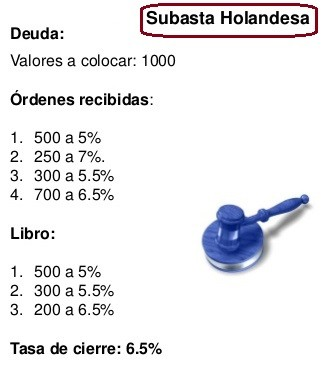
\includegraphics[scale=0.7]{photos/subasta-holandesa1.jpg}
      \caption{Ejemplo de subasta holandesa en el mercado de deuda}
      \label{dutch_auction}
    \end{figure}

\section{Blockchain} \hspace*{}
  Las subastas tradicionales usualmente requieren una tercera persona, ya sea un subastador o una 
  casa de subastas que maneje el proceso completo de subasta, lo cual puede llegar a tener muy altos
  impuestos por comisiones. También sufren de un punto de fallo, los subastadores pueden en ocasiones 
  tener malas intenciones \parencite{wu2019}. En este contexto, blockchain surge como una plataforma descentralizada que
  puede ser empleada para aplicaciones de subastas en línea confiables. En 2018 por primera vez en el 
  mundo una colección de arte valuada en varios millones de dólares perteneciente a Andy Warhol fue tokenizada
  y subastada satisfactoriamente usando la blockchain de Ethereum\parencite{wood2021}\parencite{emem}. Es también
  conocido que una de las mayores casas de subastas (e.g., Sotheby’s and Christie’s) está activamente
  trabajando en aplicar blockchain para subastas seguras y confiables. \parencite{neuendorf2018}

  % On the one hand, traditional centralized auctions usually require a third-party auctioneer or auction 
  % house to manage the entire auction process, which is expensive due to high commission fees. They also 
  % suffer from a single point of failure, as auctioneers can potentially be malicious in some cases [11]. 
  % In this context, blockchain has emerged as a decentralized platform to support trustworthy online 
  % auction applications. In 2018, for the first time in the world, multi- million dollar artworks by Andy 
  % Warhol were tokenized and auctioned successfully using the Ethereum blockchain [12],[13]. It is also 
  % reported that major auction houses (e.g., Sotheby’s and Christie’s) are actively working on applying 
  % blockchain in secure and trusted auction use cases [14].

  La tecnología blockchain elimina efectivamente los intermediarios, por lo tanto, reduce los costos de 
  transacción y asegura la confianza entre las partes interesadas en la subasta. En general, la tecnología
  blockchain puede mejorar las subastas en los siguientes aspectos:
  
  - Inmutabilidad de las transacciones de la subasta. Cada transacción ejecutada en la blockchain es pública, verificable e inmutable.
  Esto significa que la blockchain puede ser empleada como dispositivo de certificado de auditoría que previene que los participantes
  hagan trampa durante la subasta. El ganador puede usar la blockchain como prueba de la transacción.
  
  - Automatización del proceso de subasta. Un contrato inteligente automatiza el proceso de la subasta en la blockchain. Casi toda 
  la lógica de la subasta puede ser predefinida en contratos inteligentes para facilitar el intercambio de bienes y servicios, así como
  el pago de los tokens.

  - Descentralización del manejo de la subasta. No hay necesidad de designar una tercera persona como subastador, que asegure la 
  confiabilidad. Las tradicionales subastas centralizadas pueden ser muy costosas y sujeta a posibles subastadores tramposos; casas
  de subastas típicamente cargan del 8 al 20\% como comisión. 

  - Flexibilidad en el pago de la subasta. Las criptomonedas existentes en la blockchain pueden mejorar la seguridad y flexibilidad
  del pago de la subasta. Al mismo tiempo, un sistema de pago descentralizado, no necesita de intermediarios financieros, haciendo
  las transacciones más convenientes y menos costosas. \parencite{shi2021} %page 6

  \subsection{Quorum} \hspace*{}

    Blockchain es de los términos más usados en el mundo de la tecnología en estos días. Mientras esta tecnología es el elemento núcleo 
    de las criptomonedas que están llegando a los mercados financieros, su uso no es limitado a las criptos y tiene muchos más casos de uso.
    Con el pasar de los años, diferentes plataformas blockchain han sido desarrolladas con sus propios mecanismos de consenso y métodos de
    encriptación.

    Una de estas plataformas es la blockchain de Quorum, la cúal ha ganado popularidad en los últimos tiempos. Esto es a causa de la larga
    lista de casos de uso que quorum provee a sus usuarios. La red de Quorum está basada en una bifurcación de la blockchain de Ethereum.
    Es un protocolo blockchain de \href{https://github.com/ConsenSys/quorum}{código abierto} especialmente diseñado para usar en redes blockchain privadas. Algo a destacar de esta red
    es su nueva característica llamada \textit{"private transaction identifier"}  que asegura la privacidad de los datos. El objetivo de
    construir Quorum es utilizar la tecnología existente tanto como sea posible. Por lo tanto, incluso si la red Ethereum se somete a 
    diferentes actualizaciones en el futuro, habría pocos o ningún cambio en la blockchain de Quorum para mantener la sincronización entre
    estas redes. 
    % https://www.lcx.com/a-guide-to-quorum-blockchain/

    % Quorum fue creada por el super banco JPMorgan Chase, pero en 2020 fue adquirida la plataforma por ConsenSys empresa de tecnología de
    % sofware blockchain fundada por Joseph Lubin y con sede en la ciudad de New York. Por esa razón en ocasiones se le llama a la 
    % blockchain como ConsenSys Quorum
    % https://www.coindesk.com/business/2020/08/25/consensys-acquires-jpmorgans-quorum-blockchain/

  \subsection{Subastas a ciegas sobre blockchain} \hspace*{}
    Las subastas sobre blockchain han sido una área centro de muchas investigaciones en los últimos años.
    Razón por la cual ya se han desarrollado algunos protocolos de subastas a ciegas sobre 
    blockchain. Algunos de los cuales son:

    - \cite{hawk2016}

    - \cite{blass2017strain}

    - \cite{galalyusef2018}

    - \cite{sanchez2020}

    - \cite{sharma2021}

    - \cite{li2021}

\chapter{Propuesta}\label{chapter:proposal}

En este capítulo se mencionará qué es lo que necesita el algoritmo buscado para ejecutar una variante de 
subasta holandesa
a ciegas sobre \textit{blockchain}, en este caso para una red \textit{blockchain} basada en Ethereum, se 
explicará porque los protocolos de la literatura no son útiles para este caso particular y se 
describirá el algoritmo implementado, programado en el lenguaje de programación Solidity. Este algoritmo 
se hace con la finalidad de facilitar y realizar de manera segura la venta de bonos soberanos para el 
mercado de deuda pública. 

\section{Requerimientos del contrato inteligente}
  Para poder ejecutar la subasta deseada es necesario que el contrato inteligente que se utilice cumpla
  unos requerimientos mínimos que garanticen la ejecución satisfactoria y completa del proceso de subasta.
  Estos requerimientos son:

  \begin{itemize}
    \item Seguridad y completitud del proceso de subasta. A este requerimiento contribuye que el proceso de
    subasta se efectúe en la \textit{blockchain}, pero también se hace necesario que el algoritmo implementado
    no tenga brechas de seguridad.
    \item Descentralización. Para que la subasta sea descentralizada no se puede depender de confiar en un
    subastador o tercera persona. Es necesario que ninguno de los participantes en la subasta, ni siquiera
    el que oferta los bonos, tenga acceso a información privilegiada.
    \item Ocultar el precio de las ofertas. Se hace necesario para que la subasta sea a ciegas, que
    no se sepa la información de las ofertas realizadas.
    \item Ofertas con múltiples parámetros. En el caso de las ofertas hechas 
    en la subasta objetivo (la que se quiere ejecutar) cada oferta está compuesta por dos valores
    enteros, los cuales son porciento y cantidad. 
    \item Posibilidad de efectuar múltiples ofertas. Se hace necesaria la posibilidad de enviar varias 
    ofertas; normalmente en las subastas a ciegas se efectúa una sola oferta. Pero en este caso, como
    las ofertas presentan dos parámetros, es imprescindible que se puedan realizar múltiples ofertas,
    con diferente porciento de interés.
    \item Múltiples ganadores. Como en la subasta no se quiere vender un artículo, sino que se subastan 
    bonos, es muy probable que haya múltiples ganadores (a cada ganador se le otorgaría
    cierta cantidad de bonos), y no solo uno como en subastas tradicionales.
  \end{itemize}

  \subsection{Protocolos para subastas a ciegas}
    Como se vio en la sección \ref{section:blind_auction_protocols}, en la cual se hizo un pequeño resumen
    de cada protocolo, estos presentan algunos inconvenientes para las subastas a ciegas.
    Pero al ser la subasta requerida, una variación de la subasta a ciegas tradicional, a continuación
    se hará un análisis para determinar si esos protocolos anteriormente vistos cumplen los requerimientos necesarios
    para resolver el problema actual.

    \begin{itemize}
      \item Kosba et al. (\citeyear{kosba2016hawk}) y su propuesta Hawk: si bien pudieran cumplir casi
      todos los requerimientos, no sería de manera descentralizada. Pues siempre va a depender de una
      tercera persona de confianza que haga de subastador y no revele información sensible.

      \item Blass and Kerschbaum (\citeyear{blass2017strain}) y su propuesta Strain: en este caso falla
      el requerimiento de seguridad, dado que si alguno/os de los participantes de la subasta se retira,
      o muestra la información de su oferta, la subasta puede quedar comprometida (debido a que las 
      llaves privadas están parcialmente compartidas entre todos los participantes) y termina 
      tempranamente, sin haber concluido completamente.

      \item Galal and Youssef (\citeyear{galalyusef2018a}): necesita de una tercera persona, no participante
      en la subasta, que actúe como subastador. Comprometiendo así la descentralización de la subasta y el
      riesgo a que este subastador filtre información.
      
      \item Sánchez (\citeyear{sanchez2020}): propuso Raziel, el cual hace viable la privacidad y la
      verificabilidad de varios tipos de aplicaciones, entre los cuales está la subasta a ciegas. Pero
      se hace difícil y complicada la adaptación del algoritmo a múltiples ofertas y múltiples ganadores.

      \item Sharma et al. (\citeyear{sharma2021}): la propuesta realizada se basa en que existe 
      una \textit{blockchain} que permite transacciones anónimas y confidenciales. En el caso de la 
      \textit{blockchain} de Ethereum esto no se cumple, por lo tanto, esta propuesta no funcionaría como debería
      en algunas \textit{blockchain}.

      \item Li and Xue (\citeyear{li2021}): en este caso, este protocolo tiene una dificultad en cuanto al
      tiempo, pues, depende de la cantidad de postores (ofertantes) que participen en la subasta. Mientras
      más participen, mayor será el tiempo que se tome en ejecutarse el algoritmo. Dificultando el proceso
      de subasta en caso de tener esta muchos participantes.

    \end{itemize}

    En resumen, todos los protocolos revisados, presentan problemas para cumplir los requerimientos del
    algoritmo necesitado. En general, las principales dificultades son la no descentralización total del 
    contrato, haciéndole dependiente de un subastador de confianza y la necesidad de tener varios 
    ganadores y varias ofertas en la subasta, para la cual estos protocolos no están destinados.

\section{Ventajas de la propuesta}
  Los esquemas y protocolos para subastas a ciegas de la literatura consultada no cumplen con los
   requerimientos necesarios
  para resolver el problema en cuestión (subasta a ciegas de bonos soberanos) o se hace difícil su 
  adaptación al problema a resolver.
  Dado esto, se propone una solución que se adapta a los requerimientos del problema y que además es 
  segura y confiable.

  Ventajas

  \begin{enumerate}
    \item No es necesario que los participantes de la subasta se registren en esta. Para participar solamente necesitan hacer dos 
    transacciones, la oferta y luego la revelación de la oferta.
    \item Posibilidad de hacer varias ofertas. Cada participante o postor de la subasta puede realizar cuantas ofertas estime convenientes,
    no tiene limitantes en cuanto al número de ofertas.
    \item Permite retractar o cancelar ofertas. En la fase de revelación, el usuario puede decidir no proceder con una oferta.
    \item Admite múltiples ganadores. Los bonos se reparten entre los ganadores de la subasta, que en la mayoría de los casos será más 
    de uno. 
  \end{enumerate}

  A pesar de las ventajas de la propuesta, también se presentan algunas desventajas, las cuales se describen en el siguiente apartado. 
  
  Desventajas:

  \begin{enumerate}
    \item Las ofertas son reveladas. Si bien en la fase de ofertas estas son desconocidas, es necesario revelar la información real de la oferta para comprobar su validez.
    \item Posibilidad de colisión. Al utilizar un algoritmo de \textit{hash} para codificar las ofertas, existe la posibilidad (aunque bastante
    poco probable) de que la información de dos ofertas diferentes, den el mismo \textit{hash}. 
  \end{enumerate}

  Teniendo en cuenta que las desventajas no son significativas y que la seguridad y confiabilidad de la 
  subasta se mantienen en un nivel alto; Y, por el contrario, presenta
  ventajas muy beneficiosas para resolver la problemática, incluso, alguna de ellas no vistas en los esquemas de subasta que se han investigado con anterioridad. El autor considera como factible la implementación de esta proupuesta.

\section{Condiciones iniciales}
  Con el propósito de ganar en comprensión y lograr mayor especificidad en algunos asuntos, en lo adelante la propuesta estará enfocada a la \textit{blockchain} de Ethereum, y todo lo que se refiera a la implementación e interacción del contrato inteligente a partir de ahora, va a estar enfocada a esta \textit{blockchain} en particular. A pesar de esto, la propuesta implementada se podrá utilizar en la red de Quorum o en otras redes basadas
  en Ethereum sin ninguna o muy pocas modificaciones.

  Para participar en la subasta como postor solo es necesario tener una cuenta en la \textit{blockchain} de Ethereum, la aplicación o extensión
  Metamask (o alguna otra que permita interactuar con contratos inteligentes) y una cantidad de ether suficiente para pagar la comisión
  de gas de las transacciones.

\section{Proceso de Subasta}
  El proceso de la subasta va a estar compuesto por cinco fases principales: despliegue, ofertas, revelación,
  verificación y finalización.

  A partir de este momento al que oferta los bienes a subastar (en este caso los bonos) se le llamara  \textbf{beneficiario} (para el problema en cuestión sería el gobierno) y al que despliega el contrato inteligente en la \textit{blockchain} le llamaremos \textbf{subastador} (a pesar de que no cumple el mismo objetivo ni funciona como los subastadores tradicionales). El beneficiario y el subastador pueden ser una misma persona, o tratarse de personas diferentes. Por último, a los participantes en la subasta se les llamará \textbf{postores}. Para mayor comodidad, beneficiario, subastador y postores van a ser los usuarios de la subasta.

  \subsection{Desplegar contrato}
    El contrato inteligente puede ser desplegado a la \textit{blockchain} por el propietario de lo que se oferta
    o por una tercera persona que haga función de subastador. Esta persona no tiene ningún poder, ningún
    privilegio en el contrato inteligente, ni tampoco tiene acceso a retirar los activos del contrato. La única función del subastador 
    es la de poner los parámetros iniciales de esta, dígase: 
  
    \begin{enumerate}
      \item boneToSale: valor total de los bonos que se quieren vender;
      \item biddingTime: tiempo de duración de la fase de ofertas;
      \item revealTime: tiempo de duración de la fase de revelación de ofertas;
      \item beneficiaryAddress: dirección donde se quiere recibir el pago de los bonos vendidos.
    \end{enumerate}

    Cada vez que se quiere hacer una nueva venta de bonos, es necesario volver a desplegar el contrato inteligente.

  \subsection{Fase de ofertas}
    Cada postor puede realizar cuantas ofertas estime convenientes. Dado que lo que se oferta en la subasta son bonos (como se explicó anteriormente, son una especie de préstamos por tiempo definido que se le hace al gobierno), cada puja está compuesta de dos partes: la cantidad que el postor está dispuesto a prestar y cuál sería el interés a cobrar por ese préstamo en porciento. 

    Dada la necesidad de que las ofertas no sean conocidas por los demás postores, luego de escoger las condiciones de la oferta a efectuar, en vez de enviar los datos reales de esta, el postor codifica esa información (cantidad y porciento) en conjunto con una palabra secreta solo conocida por él, y tal codificación es lo que se envía al contrato inteligente. Es importante destacar que la cantidad enviada en la transacción, en conjunto con la codificación de la oferta, no tiene que ser necesariamente la cantidad exacta de la oferta enviada, esta cantidad se deposita en el contrato inteligente y se añade al saldo de esa dirección en el contrato, para un posible uso posterior de este en ofertas venideras.

    Para codificar la oferta se hace uso de la función de Solidity: \textit{keccak256}, la cual es un 
    algoritmo o función de \textit{hash} que toma como entrada un conjunto de datos y devuelve un valor de 
    longitud fija, 32 \textit{bytes}. Esta función es una de las más utilizadas en la programación de contratos 
    inteligentes, ya que permite la creación de \textit{hash} de datos que no pueden ser revertidos a su 
    valor original, es decir, que no se puede obtener la información original de un \textit{hash}. 
    En este caso, \textit{keccak256} es empleada para codificar la oferta, por lo que no se puede saber la 
    cantidad y el porciento de la oferta que se realizó.

    Luego de desplegado el contrato inteligente hay un tiempo hábil para mandar ofertas, después de ese tiempo no serán recibidas más ofertas. Y da inicio a la fase de revelación de ofertas.

    \subsection{Revelación de ofertas}
    Cada postor que realizó ofertas debe enviar al contrato la información de las que quiere revelar. Es decir, tiene que enviar tres arreglos, que van a representar valor, porciento y palabra secreta de las ofertas, respectivamente. Es necesario que el tamaño de los arreglos sea igual a la cantidad de ofertas enviadas, de lo contrario, no serán analizados, y será necesario una nueva transacción con la información completa. La posición del arreglo significa el número de la oferta, ordenada por tiempo de recepción en el contrato inteligente. 
    
    El contrato inteligente se encarga de codificar la información suministrada, con la misma función \textit{keccak256} que fue utilizada por el postor, y la comprueba con la codificación enviada por este, en la fase de ofertas. Si las dos codificaciones coinciden exactamente, quiere decir, que los datos de la oferta son los mismos que el postor eligió en la fase de ofertas, y por tanto, se considera válida. Para que la oferta sea totalmente válida, es necesario que el valor depositado hasta ese momento en el contrato sea mayor o igual que el valor de la puja de esa transacción. A cada oferta válida se le asigna un identificador único $id$, por orden de revelación (las ofertas que primero se revelan tienen un menor $id$), que posteriormente será usado.

    Si la oferta no es válida, ya sea por no coincidir los valores \textit{hash} de las codificaciones o por no tener suficiente dinero disponible para ejecutar la oferta, se anula la oferta; sin embargo, el dinero depositado en esa transacción queda disponible para próximas ofertas, aunque también disponible para retirar en cualquier momento posterior. Cuando se solicita un retiro (\textit{withdraw}) del contrato, si la dirección que lo solicita tiene algún fondo disponible para retiro, recibe el reembolso de todo lo disponible en el contrato.

    Es necesario destacar que la revelación de las ofertas ocurre solamente una única vez por cada dirección, es decir, si una oferta es considerada válida o no válida (por alguna de las razones vistas anteriormente), pues no hay forma de cambiar ese veredicto. Por esto es necesario tener sumo cuidado con la información que se envía al contrato inteligente, tanto en la fase de ofertas como en la fase de revelación, ya que una vez que se envía, no hay forma de cambiarla.

  \subsection{Verificación y publicación de los ganadores}
    En esta fase, se comprueba cuáles son los ganadores de la subasta y se publican los resultados. Para esto, ya se tienen las ofertas válidas, determinadas por la fase de revelación, estas se ordenan crecientemente por el porciento de interés que ofrecen, es decir, las que a menor porciento de interés tienen el préstamo, van primero, dado que son las más convenientes para el deudor. En caso de tenerel mismo porciento se desempata por la oferta con menor id. 

    Luego de ordenadas las ofertas, se comienzan a aceptar hasta lograr la cantidad total que se necesita para cubrir el valor
    de los bonos ofertados. Para esto, se comienza con la oferta con menor porciento de interés, 
    y se acepta la oferta, es decir, disminuye la cantidad de bonos ofertados. Luego se pasa a la siguiente oferta, y se acepta la oferta, 
    y así sucesivamente hasta que se agoten los bonos ofertados o hasta agotar todas las ofertas válidas.

    A todos los ganadores de la subasta se les paga un único porciento de interés, el de la última oferta aceptada, es decir, de la oferta aceptada con mayor porciento de interés.

    En caso de que para un porciento de interés se tengan varias ofertas con ese mismo porciento, se acepta primero la oferta con menor id. Por consiguiente, si en el último porciento de interés aceptado se tienen varias ofertas, el desempate está dado por el tiempo de revelación de la oferta (que es lo que determina el id de la oferta). Esto estimula a los postores a revelar sus ofertas lo más pronto posible, para tener mayor probabilidad de estar entre los ganadores de la subasta.

    En caso de que la última oferta aceptada sobrepase la cantidad de bonos ofertados, se acepta la oferta parcialmente, es decir, se
    acepta solamente la cantidad que se necesita para cubrir el valor de los bonos ofertados.

    Luego de que ya se tienen las ofertas ganadoras, el dinero bloqueado de las ofertas restantes (si quedara alguna) es puesto a 
    disposición de sus respectivos postores, para que puedan retirarlo.

    \subsection{Finalización}
    Esta fase está estrechamente ligada con la anterior, se hacen una a continuación de la otra. Para su mejor comprensión, se le destinó una fase independiente. En esta fase, se publican los resultados de la subasta, es decir, se publican las ofertas ganadoras (dirección, porciento y cantidad a prestar de cada una). Además, se publica el porciento de interés que se le pagará a los ganadores. Y seguidamente se transfiere el dinero de los postores ganadores, en este caso convertidos en prestamistas, a la dirección del beneficiario de la subasta, que sería el deudor de los préstamos.

    Por último el contrato inteligente activa una bandera que indica que la subasta ya ha finalizado, y que no se pueden hacer más
    ofertas, ni revelaciones, ni nada relacionado con la subasta, solamente retiros del dinero de los postores que tengan dinero disponible.

    El contrato fue diseñado para subasta de bonos soberanos, pero puede ser empleado para cualquier otra subasta del mercado de deuda.
    Y también puede ser fácilmente adaptado para realizar otro tipo de subastas.

\section{Seguridad}
  \subsection{Obligación de pago del beneficiario}
    En la implementación realizada, se asume la fiabilidad del beneficiario de la subasta, a la postre deudor. No se llega a implementar ninguna medida para asegurar el pago a los prestamistas, dado que depende mucho de las condiciones de la subasta y se escapa un poco del alcance que pudiera tener el contrato inteligente. Sin embargo, se expondrán a continuación algunas propuestas, que pudieran ser empleadas para garantizar o al menos mejorar la confianza de los postores hacia el beneficiario.

    \begin{enumerate}
      \item El beneficiario tiene que depositar algún activo como colateral en el contrato inteligente, que sea igual al valor total o al menos
      a los intereses a pagar por los bonos que
      se ofertan. De esta manera, si el beneficiario no paga, el contrato inteligente puede pagar a los prestamistas con el dinero
      depositado por el beneficiario.
      \item Liberación de fondos en partes. En lugar de liberar el dinero de los prestamistas al final de la subasta, se puede liberar el 
      dinero de los prestamistas en partes, es decir, liberar el dinero de los prestamistas en partes, proporcionalmente a los intereses 
      que se
      van pagando. De esta manera, si el beneficiario no paga, el contrato inteligente puede pagar a los prestamistas con el dinero
      congelado en el contrato inteligente.
      \item Tokenizar los bonos. En lugar de ofertar los bonos, se puede ofertar tokens que representen los bonos. De esta manera, estos tokens servirían como garantía de que el beneficiario pagará los intereses de los bonos. Quizás hasta se podrían legalizar estos tokens, de manera de que se pudiera incurrir en acciones legales en caso de que el beneficiario no pague los intereses de los bonos o la devolución total  del préstamo luego del vencimiento de este. Estos tokens pudieran también servir para que los prestamistas puedan vender sus tokens en el mercado secundario, y así recuperar parte de su dinero invertido. Se crearía así un mercado secundario para los bonos, que es algo que no existe en el mercado de deuda cubano actualmente y que fomentaría la liquidez de los bonos y el interés de los inversores en estos.
    \end{enumerate}

    El autor opina que cada una de estas opciones puede ser viable en algún caso particular. Desde su punto de vista, la mejor y más conveniente opción es la tercera, ya que es la que mejor garantiza el pago de los intereses y la devolución del préstamo, y además, tiene múltiples beneficios adicionales, para los prestamistas y el mercado de deuda cubano en general.

  \subsection{Keccak256}
    El algoritmo Keccak, se basa en el término criptográfico de construcción de esponja, en este caso 
    Keccak a partir de una entrada de cualquier longitud, le aplica una función $F$ y obtiene como resultado 
    una salida de cualquier longitud deseada. Esto provoca una gran flexibilidad \parencite{bertoni2007}.

    El algoritmo Keccak es el trabajo de Guido Bertoni, Joan Daemen, Michael Peeters y Gilles Van Assche. Está basado en los diseños de 
    \textit{hash} PANAMA y RadioGatún. En el año 2006, el \textit{National Institute of Standards and Technology} (NIST) organizó una nueva edición de la competición para la creación de una nueva función 
    para los estándares de Secure Hash Algorithm (SHA), el SHA-3. Al no existir un ataque significativo demostrado en SHA-2, el nuevo 
    estándar SHA-3 no lo reemplazará. La NIST ha mencionado que debido a exitosos ataques a los estándares MD5, SHA-0 y SHA-1, es 
    necesario una alternativa llamada SHA-3 \parencite{stevens2017}.

    Las admisiones de proyectos comenzaron en el año 2008. Keccak fue aceptado como uno de los 51 candidatos. En julio de 2009, 14 
    algoritmos pasaron a la segunda ronda y Keccak avanzó a la ronda final en diciembre de 2010. Durante el periodo de la competición, se 
    les permitió a los participantes corregir problemas descubiertos en sus algoritmos. Keccak hizo algunos cambios como el número de 
    rondas, se amplió de ${\displaystyle 12-\ell}$ a ${\displaystyle 12-2\ell }$. En 
    octubre de 2012 fue seleccionado como el ganador de la competición. En el año 2014, la NIST publicó la documentación técnica del 
    algoritmo y fue aprobado en agosto de 2015, para así convertirse en el nuevo estándar SHA-3 \parencite{nist2015}.

    En el caso de Bitcoin, el uso del algoritmo de \textit{hash} SHA256 está bastante extendido,
    además es utilizado en multitud de implementación de funcionalidades de la cadena
    de bloques de Bitcoin. En cambio, Ethereum hace uso del algoritmo de \textit{hash} Keccak-
    256, aprobado por la NIST en agosto del 2015, convirtiéndose en el nuevo estándar
    SHA-3.
    Cabe destacar que debido a que la aprobación por parte del NIST de este algoritmo fue más tardía que el desarrollo de Ethereum, el 
    estándar final de SHA-3 adoptado por la NIST hace referencia al estándar “FIPS-202 SHA-3”, el cual sufrió ligeros cambios en sus parámetros, a diferencia del algoritmo Keccak-256 implementado en Ethereum.

    \begin{verbatim}
  Keccak256("")
  = c5d2460186f7233c927e7db2dcc703c0e500b653ca82273b7bfad8045d85a470

  SHA3("")
  = a7ffc6f8bf1ed76651c14756a061d662f580ff4de43b49fa82d80a4b80f8434a
    \end{verbatim}

    Como se produjeron ligeros cambios en el SHA-3 (con respecto al Keccak-256) antes de su aprobación por el NIST, las salidas de estos algoritmos no son iguales entre sí en el caso de que haya entradas iguales. Para comprobarlo, como se hace en el ejemplo anterior, se puede observar los valores en ambos casos de uno entrada vacía, lo que da como resultado dos salidas distintas. Por lo tanto, a pesar de que en múltiples papers y documentos de Ethereum se haga referencia a SHA-3, realmente se quiere hacer referencia al uso de Keccak-256 \parencite{taibo2022}.

    % other post: https://www.geeksforgeeks.org/difference-between-sha-256-and-keccak-256/

% \chapter{Experimentación y Resultados}\label{chapter:implementation}

En este capítulo se explica cómo se desarrollaron los experimentos realizados, los elementos que formaron 
parte de los mismos, además se se enuncian y justifican algunas de las decisiones tomadas en la implementación
del algoritmo. Por último, se analizan los resultados obtenidos, y si es factible o no la propuesta
para el problema que se quiere resolver.

\section{Detalles de Implementación}
  En la fase de revelación de ofertas se van verificando estas y a la par se van construyendo dos arreglos con las ofertas válidas. Uno de estos arreglos \textit{bidsRevealed} contiene 
  \textit{<value, percent, biderAddress>} (valor, porciento y dirección del postor) de cada oferta. Y
  el otro arreglo \textit{bidsRevealedPercentID} solo contendrá \textit{<percent, id>} (porciento e 
  identificador numérico) de cada oferta válida, cabe destacar que este \textit{id} es la posición del
  arreglo donde se encuentra la oferta, esta información será utilizada más adelante.

  Para determinar los ganadores de la subasta, es necesario seleccionar las mejores ofertas. Para el
  problema actual, que es una variación de la subasta holandesa, las ofertas que ofrecen menores
  porcientos de interés serán las ganadoras. Para escoger estas ofertas, se ordena el arreglo
  \textit{bidsRevealedPercentID}, donde el porciento va a ser el valor por el que se va a hacer el 
  ordenamiento de forma ascendente (de menor a mayor valor). En caso de dos ofertas con igual porciento
  se definirá su orden en dependencia de la que menor \textit{id} tenga.

  Para ordenar el arreglo se hace uso del algoritmo Quick Sort. ¿Por qué se usó Quick Sort y no otro 
  algoritmo de ordenamiento? A pesar de que este algoritmo puede llegar a tener en su peor caso costo
  computacional $O(N^2)$, en el caso promedio se comporta como un algoritmo cuasi lineal $O(N log N)$.
  No se empleó el \textit{merge sort} por la complejidad del lenguaje Solidity en el manejo de la memoria
  y las variables a utilizar, que se deben a las particularidades de la blockchain como nueva tecnología.
  El \textit{merge sort} necesita de un arreglo adicional para ejecutarse y generaría costo 
  computacional adicional, por esta razón no es conveniente su uso. Otra posible opción era el Heap Sort 
  (que no necesita memora adicional), pero 
  se prefirió el empleo del Quick Sort, por la sencillez de su implementación.

  \section{Experimentación}
  \subsection{Tecnologías utilizadas}
    El contrato inteligente que procesa la subasta fue programado en el lenguaje Solidity v0.8.4 
    \parencite{solidity0.8.4}. Para las pruebas realizadas al contrato se utilizó Python 3.8.10 
    \parencite{python3.8} en conjunto con Brownie v1.19.2, este último es un framework basado en Python
    para desarrollar y testear contratos inteligentes dirigidos a ejecutarse en la Máquina Virtual de 
    Ethereum. Además, se empleó Ganache v7.5 \parencite{ganache7.5}, una implementación local de la blockchain de Ethereum, que permite llevar a cabo pruebas de contratos inteligentes sin necesidad de tener una red
    real de Ethereum.

    \subsection{Gas}
      Uno de los conceptos más importantes en el mundo de Ethereum es el Gas. Es una unidad de medida utilizada para medir el trabajo realizado por Ethereum para realizar transacciones o 
      cualquier interacción dentro de la red.


      Una forma sencilla para comprender qué es el Gas en Ethereum sería la siguiente analogía: se quiere viajar 
      de Madrid a Barcelona, el viaje se hará en coche. Se sabe de antemano que son 
      500 km de distancia y que el coche gasta 1 litro de gasolina cada 10 km (para hacer simple el cálculo), 
      así que se necesitará 50 litros de gasolina para llegar al destino. Además, también se sabe que el 
      litro de gasolina cuesta entre 1 € y 1,5 € dependiendo de la gasolinera donde se detenga a repostar.


      Esto es lo mismo que pasa en Ethereum. Por un lado, cada tarea en Ethereum tiene un coste específico 
      y no variable estipulado en Gas, lo que es equivalente al litro de gasolina que gasta el auto por cada 
      10 Km. Por supuesto, las operaciones en Ethereum están formadas por distintas funciones más pequeñas, 
      cada una de ellas con un valor de Gas (o consumo de gasolina) específico y su sumatoria es lo que 
      dirá el valor final en Gas de dicha operación (el total de gasolina a gastar para hacer el viaje).
      Solo resta por responder una interrogante: ¿cuánto se pagará por ese Gas para poder llevar a cabo la operación en Ethereum?

      En la analogía anterior, la gasolina varía entre 1 y 1,5, se puede escoger dónde repostar y pagar lo 
      menos 
      posible para adquirir los 50 litros de gasolina que se necesitan para el viaje. Lo mismo pasa en 
      Ethereum, el Gas tiene un precio en Ether que es dado por la demanda y oferta de operaciones en 
      Ethereum. Es decir, el precio del Gas en Ether es variable, aunque en este caso se puede elegir el 
      valor que se va a pagar por ese Gas, y si un minero está de acuerdo con ese valor, tomará la 
      transacción y la ejecutará.

      Hay tres cosas que son importantes y vitales dentro de Ethereum, y que explicamos a continuación:

      \begin{enumerate}
        \item Unidad de Gas. La Unidad de Gas es la cantidad de Gas que se puede atribuir a una instrucción 
        en específico, pero no tiene ningún valor monetario.
        \item Precio de Gas \textit{gas price}. El Precio de Gas por su parte, es el pago de comisión que se hace por cada Unidad de Gas. Es el precio que se elige pagar por cada unidad y se hace usando unidades decimales de Ether, los llamados Gwei. Esta comisión es la que permite tener prioridad de atención. Si se paga más por cada Unidad de Gas que se use, más rápido los mineros tomarán la transacción y la llevarán a un bloque.
        \item Límite de Gas (\textit{gas limit}). Este es un valor que indica la cantidad máxima de Unidades de Gas que la red 
        Ethereum puede manejar en un momento dado. Es su límite máximo, y un punto que los mineros no 
        pueden sobrepasar en ningún momento.
      \end{enumerate}


      Este último límite es interesante, porque permite hacer frente al problema de la parada 
      (\textit{halting problem}). Este es un 
      problema de computación que permite saber si un programa se ejecutará en un bucle 
      infinito con solo tener a la mano la entrada de datos y su código fuente. Esta situación plantearía un 
      serio problema en la blockchain que podría llevar a una Denegación de Servicios (DoS). Sin embargo, 
      debido a que Ethereum impone un \textit{gas limit} por bloque, esto significa que ninguna operación en 
      Ethereum por compleja que sea podrá exceder jamás dicho límite \parencite{bit2meacademy}. El \textit{gas limit} actual de la red de Ethereum es de 30 Millones \parencite{ycharts}. Figura 
      \ref{figure:smart_contract_squeme}.


      \begin{figure}[h!]
        \centering
        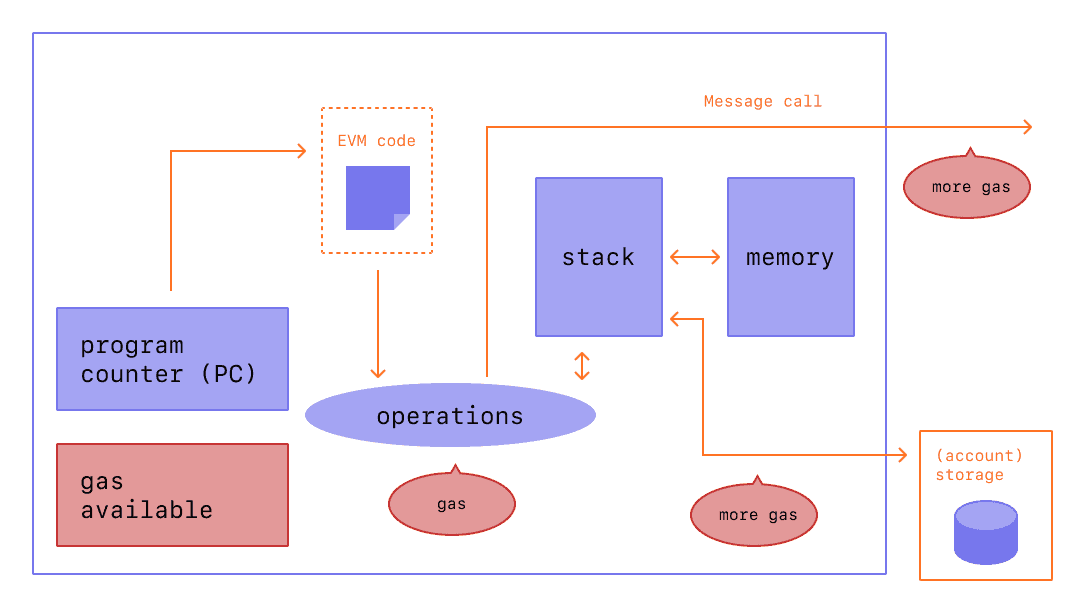
\includegraphics[scale=0.4]{Graphics/gas.png}
        \caption{Diagrama resumen, sobre funcionamiento interno de un contrato inteligente}
        \label{figure:smart_contract_squeme}
      \end{figure}

      \subsubsection{Gas en Quorum}
      Por defecto, la red de Quorum (GoQuorum) es una red libre de gas, lo que significa que el gas no 
      tiene precio (\textit{gas price} igual a 0).


      Las transacciones usan recursos computacionales, por lo que tienen un costo asociado.
      Gas es la unidad de costo y \textit{gas price} es el precio por cada unidad de gas. El costo de
      una transacción es la cantidad de gas empleado multiplicado por el precio del gas. 
      
      En redes públicas como Ethereum, la cuenta que envía la transacción paga el costo de la transacción,
      en Ether. El minero (o validador, en redes con prueba de autoridad) que incluye la 
      transacción en un bloque recibe el costo de la transacción como recompensa.


      En muchas redes privadas, incluyendo GoQuorum, los participantes de la red ejecutan los 
      validadores y no requiere gas como incentivo (como pasa en las redes públicas). Las redes que no 
      requieren gas como incentivo usualmente eliminan el precio del gas o lo configuran para que sea cero
      (gas gratis). Algunas redes privadas pueden distribuir Ether y utilizar un \textit{gas price}
      diferente de cero para limitar el uso de recursos.


      En redes libres de gas, el precio del gas es cero, aunque las transacciones se mantengan usando gas,
      por consiguiente, el costo de la transacción (gas usado por el precio del gas) es cero.


      En GoQuorum, el precio del gas es completamente removido a menos que sea explícitamente habilitado.
      El precio del gas no está incluido entre los parámetros del objeto transacción en los métodos de la
      API privada de GoQuorum \parencite{consensysfreegas}.


      Con lo visto anteriormente se puede concluir que el gas no es totalmente necesario en GoQuorum, ya 
      que no se requiere como incentivo para los mineros, por lo tanto, no se paga por las transacciones
      realizadas en GoQuorum. No obstante, el gas sigue siendo importante para el funcionamiento de
      los contratos inteligentes, por el hecho de que indica la cantidad de recursos computacionales que se requieren para ejecutar una transacción. Y con esto, se puede saber si el algoritmo es eficiente y  escalable. En la siguiente sección se estará abordando este tema.

      \subsection{Pruebas Realizadas}
      Se realizaron varias pruebas al contrato inteligente, para verificar su funcionamiento. En las pruebas 
      iniciales se comprobó que el contrato se desplegara correctamente, y que se pudieran efectuar las 
      transacciones de manera correcta. Luego se hicieron varias pruebas con diferente cantidad de 
      postores y estos a su vez con varias ofertas (válidas e inválidas). La cantidad de postores se 
      escogía de forma aleatoria entre 1 y 12; la cantidad de ofertas de cada postor, también aleatoriamente, entre 1 y 10 ofertas. Finalmente, se efectuaron algunas pruebas de estrés para comprobar los límites máximos de postores y el límite máximo de ofertas válidas.

      En el contrato inteligente, hay 5 métodos que necesitan de transacciones para ejecutarse. Estos son:

      \begin{itemize}
        \item deploy: desplegar el contrato. Esta transacción se lleva a cabo solamente una vez, por el 
        subastador.
        \item bid: enviar una oferta. Esta función puede ser invocada varias veces, por varios postores o por
        el mismo postor. En cada llamado a la función (transacción) se debe enviar un hash (oferta codificada)
        y opcionalmente hacer un depósito en el contrato (no tiene que ser por el mismo valor de la oferta enviada,
        puede ser más o menos que esa cantidad).
        \item reveal: revelar ofertas. Esta función se debe llamar solamente una vez por cada postor. Su
        objetivo es revelar las verdaderas ofertas y clasificarlas en ofertas válidas e inválidas.
        \item auctionEnd: elegir y anunciar ganadores y dar por terminada la subasta. En este método se
        ordenan las subastas válidas, se eligen las mejores hasta completar la totalidad de los bonos
        ofertados.
        \item withdraw: retirar fondos. Cuando se llama a esta función se retiran todos los fondos 
        desbloqueados (depósitos de ofertas inválidas o válidas no ganadoras) pertenecientes a la dirección 
        que envía la transacción.
      \end{itemize}

      En las pruebas realizadas se obtuvo que las funciones usaban la siguiente cantidad de gas para 
      ejecutarse:

      \begin{table}[h!]
        \centering
        \begin{tabular}{|c|c|} \hline
          metodo        & gas usado        \\ \hline
          $deploy$      & $1227782$        \\ \hline
          $bid$         & $[68688, 83700]$ \\ \hline
          $reveal$      & ¿?         \\ \hline
          $auctionEnd$  & ¿?         \\ \hline
          $withdraw$    & $19709$          \\ \hline
        \end{tabular}
        \caption{Gas usado por cada método}
        \label{gas_used}
      \end{table}


      En las funciones \textit{reveal} y \textit{auctionEnd} el gas usado, es variable, depende de las
      condiciones particulares de cada subasta. Tabla \ref{gas_used}.


      \begin{figure}
        \centering
        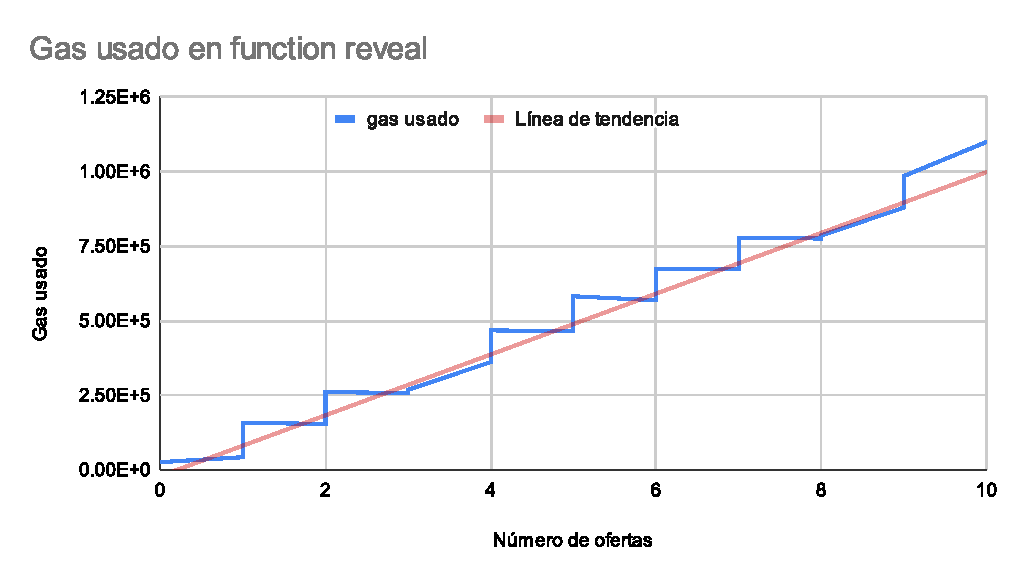
\includegraphics[scale=0.9]{Graphics/gas_reveal.pdf}
        \caption{Gas usado por la función "reveal"}
        \label{gas_reveal}
      \end{figure} 
  
      En la función \textit{reveal} el gas empleado va a depender de la cantidad de ofertas de cada postor.
      Es decir, mientras más ofertas tenga que revelar el postor, mayor será la cantidad de gas que
      consumirá esta. Figura \ref{gas_reveal}.


      \begin{figure}
        \centering
        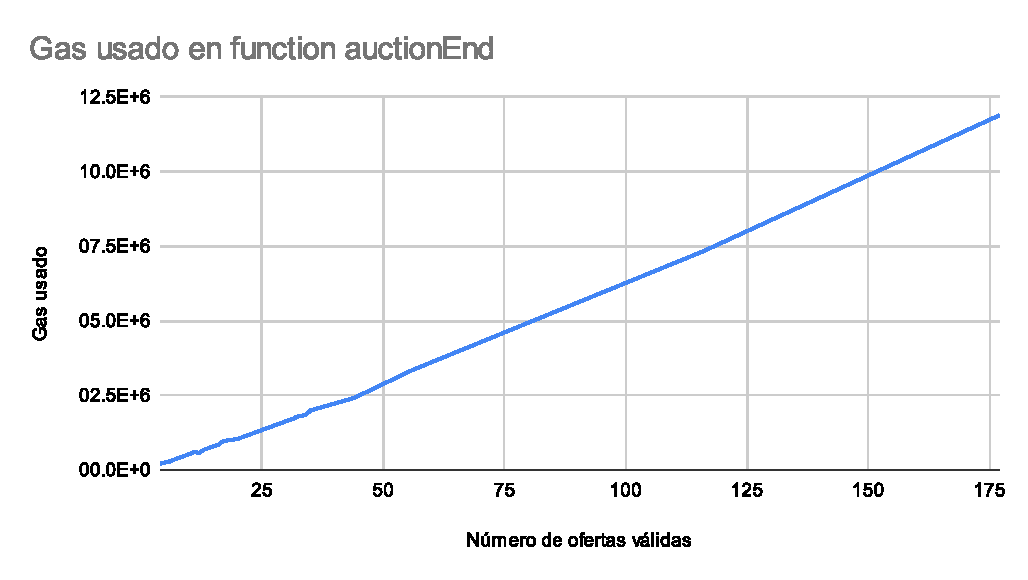
\includegraphics[scale=0.9]{Graphics/gas_auctionEnd.pdf}
        \caption{Gas usado por la función "auctionEnd"}
        \label{gas_auctionEnd}
      \end{figure} 
  
      En la función \textit{auctionEnd} pasa algo similar a la anteriormente vista. El gas empleado va a 
      depender en este caso de la cantidad de ofertas válidas. Es decir, mientras más ofertas válidas tenga 
      la subasta mayor será la cantidad de gas consumido por esta función. Figura \ref{gas_auctionEnd}.


      Para los dos casos anteriores, el gas usado depende cuasi linealmente de la cantidad de ofertas del 
      postor y de la cantidad de ofertas válidas, es decir, si los datos de entrada se duplican, el gas 
      empleado también se duplica.


      En la red local desplegada para probar el contrato inteligente, el límite de gas por bloque es de 
      12 millones (12M) de unidades. Dado este límite y las pruebas de estrés que se le hicieron al 
      algoritmo en esta red local, los límites máximos que las funciones permitían sin exceder el límite
      de gas, y por lo tanto, sin afectar la correcta y completa ejecución del programa, se llegó a los
      siguientes resultados: cantidad máxima de ofertas por un mismo postor fue de 110 aproximadamente,
      y la cantidad de ofertas válidas en la subasta en general de alrededor de 175 ofertas.


      El límite de gas de la red Ethereum actualmente es de 30M \parencite{ycharts}, por lo tanto, en esta red, pudieran ser mayor aún los límites de una subasta realizada con el contrato inteligente propuesto.
      Para predecir los límites en esta red, se usó un algoritmo de regresión lineal, el cual, teniendo 
      los datos de las pruebas en la red local, se obtiene un valor aproximado de cuánto consumiría una 
      ejecución con una cantidad arbitraria de ofertas. Luego de utilizado el algoritmo, el resultado que 
      se obtuvo es que en la red pública de Ethereum se podría efectuar una subasta donde cada postor 
      pusiera a lo más 290 ofertas y que el total de ofertas válidas fuera a lo sumo 440.

  \section{Resultados}
    Teniendo en cuenta los resultados obtenidos en las pruebas realizadas, el algoritmo funciona 
    correctamente y cumple con los objetivos planteados. El contrato inteligente propuesto es factible y 
    útil para ejecutar
    subastas de bonos con ofertas a ciegas en la blockchain de Ethereum o cualquier otra blockchain 
    basada en Ethereum.


    A pesar de que los resultados fueron satisfactorios, también se presentan algunos inconvenientes.
    Las funciones de revelación de ofertas y de fin de subasta, presentan mucho costo computacional para 
    ejecutarse en una blockchain, a medida que aumentan la cantidad de ofertas en la subasta, aumenta 
    proporcionalmente 
    su costo computacional y por consiguiente el gas usado, lo que impide que se ejecute correctamente el contrato
    si se excede el límite de gas de la red utilizada.


    El contrato puede ser empleado, pero a pequeña escala, es necesario que la cantidad de ofertas sea 
    limitada. Por lo tanto, la subasta se debe hacer en un ambiente cerrado, es decir, donde se tenga
    control sobre la cantidad de participantes en la subasta y/o de la cantidad de transacciones realizadas.
    
    No se recomienda ejecutar la subasta en entornos abiertos como Internet, donde muchos tengan acceso al
    contrato, pues de efectuarse un número importante de ofertas en la subasta, el contrato podría tener
    fallos en su funcionamiento y comportamientos inesperados.

\backmatter

% \begin{conclusions}
    Las subastas son un mecanismo de venta cada día más usado. Con el auge de las tecnologías de la 
    información, sistemas de pago electrónico y de un mundo interconectado, a través de internet. Cada
    vez se hace un mayor uso de subastas electrónicas. Por esta razón, se hace necesario protocolos y 
    mecanismos para incrementar la seguridad de estos sistemas y protegerlos de hackers que explotan
    vulnerabilidades de seguridad en las plataformas de subastas, pero también proteger a los usuarios
    de subastadores malintencionados que pueden terminar siendo estafadores, este último problema cada
    vez más latente en la actualidad.

    La blockchain y los contratos inteligentes, surgen luego del 2015 y la aparición de la blockchain de 
    Ethereum, como
    una herramienta eficaz para hacer frente a estos problemas, poniendo a nuestra disposición la 
    capacidad de crear transacciones y programas incorruptibles, que se mantienen públicos a la vista 
    de todos, haciendo que algunos procesos antes oscuros y cerrados, sean ahora totalmente transparentes
    y abiertos a cualquier persona.

    Gracias a esta tecnología, surge la idea de crear subastas en la blockchain, aportándole así seguridad
    y fiabilidad al proceso. Pero con esta total transparencia de la blockchain surgen algunas dificultades
    para realizar algunos tipos de subasta. ¿Cómo lograr ejecutar una subasta a ciega, si toda la información
    es pública?

    En la literatura consultada se presentan varias propuestas, casi todas relacionadas directamente
    con la criptografía para ocultar las ofertas de la subasta. En la propuesta implementada se utiliza con
    este objetivo la función \textit{hash keccak256}, la cual es altamente probada y utilizada para 
    proteger datos (en este caso ofertas de la subasta) de los demás usuarios de la subasta, incluyendo 
    el subastador.

    Para el desarrollo del contrato inteligente se utilizó el lenguaje Solidity, el cual es un lenguaje
    especializado en la creación de contratos inteligentes específicamente creado para la red de 
    Ethereum, pero que redes posteriormente creadas también han adoptado su uso.

    A pesar de no haber llegado a desplegarse el contrato en la red de Quorum, el autor cree que las
    características de esta red son ideales para desarrollar un contrato de este tipo. Como característica
    a destacar es que las transacciones realizadas en esta red, al ser una red privada y no pública (como 
    Ethereum) es que las transacciones son libres de costo, hecho que facilita la realización satisfactoria
    de todos los procesos y transacciones que requiere el contrato inteligente propuesto.

    Además, el contrato inteligente implementado, según las pruebas realizadas, necesita que la cantidad
    de ofertas sean limitadas, para un correcto funcionamiento del algoritmo y el entorno de una red
    privada como Quorum permite tener más control sobre eso, sin afectar la seguridad y cumplimiento
    total de los procesos de la subasta en el contrato.
\end{conclusions}

% \begin{recomendations}
    Luego de la investigación, la implementación y las pruebas realizadas en el presente trabajo. Se 
    proponen algunas recomendaciones para analizar e investigar en futuros trabajos.

    Se hace necesario un estudio profundo de los tipos de almacenamiento que admite Solidity y los tipos de
    datos usados para implementar el algoritmo, para optimizar el uso de la memoria empleada por el algoritmo
    propuesto, recurso muy costoso en las redes blockchain.

    Se recomienda además la implementación de un \tectit{Heap} (Monticulo) en detrimento del Quick Sort,
    para escoger las ofertas ganadoras de la subasta y hacer una comparación, para ver con cuál de los
    dos algoritmos la fase de verificación de los ganadores utiliza menos gas, y por tanto, menos recursos.

    Dado que las pruebas en la red blockchain local fueron satisfactorias, se recomienda el despliegue del
    contrato implementado en la red de Quorum y su empleo en el Mercado de Deuda Pública que se desarrolla para el Banco Central de Cuba.

    Por último, se hace necesario la implementación de un mecanismo para asegurar el cumplimiento del
    beneficiario (ofertante de los bonos) de su parte en el acuerdo. La opción recomendada y más 
    factible según el autor, es tokenizar los bonos, y darlos a los postores de las ofertas ganadoras,
    en proporción a la cantidad de bonos comprados por este.

\end{recomendations}

\printbibliography[heading=bibintoc]


\end{document}
